\section{Esercitazione capitoli 1 e 2}
\subsection{A.A. 2022/23}
\begin{enumerate}
	\item Approssimando $\pi = 3.14159265\hdots$ con $3.14$:
	\begin{itemize}
		\item qual è l’errore assoluto commesso?
		\item  qual è quello relativo?
	\end{itemize}
	(approssimare la risposta a due cifre significative).
	\item Come si definisce la precisione di macchina di un’aritmetica finita? Qual è il suo significato?
	\item Qual è la precisione di macchina della singola e doppia precisione IEEE? Dedurre il numero di cifre decimali approssimativamente disponibili per la mantissa.
	\item Cosa è il fenomeno della cancellazione numerica?
	\item Come si definisce l’ordine di convergenza di un metodo per la ricerca degli zeri di una funzione?
	\item Qual è il numero massimo di iterazioni che richiederà il metodo di bisezione per determinare la radice di una funzione assegnata con tolleranza (assoluta) $10^{-3}$, se l’intervallo di confidenza iniziale è $[33, 37]$?
	\item Derivare il metodo di Newton per la ricerca della radice di una funzione e dimostrare che esso converge quadraticamente a radici semplici.
	\item Calcolare il numero di condizionamento della radice nulla di
	\begin{equation*}
		f(x)=3e^x-2\cos{x}-1.
	\end{equation*}
	\item Definire la molteplicità di una radice. Calcolare la molteplicità della radice nulla di
	\begin{equation*}
		f(x)=e^{x^2}-1.
	\end{equation*}
	Perché il calcolo di una radice nulla è un problema malcondizionato?
	\item Scrivere una function Matlab che implementi efficientemente il metodo di Newton.
\end{enumerate}

\hrule

\paragraph{1.}\footnote{Slide 3 PDF 13.} $x = 3.14159265\hdots,\, \Tilde{x}=3.14\Rightarrow\begin{cases}
	|\Delta x|=|\Tilde{x}-x|=0.0015926\hdots\approx 1.6\times 10^{-3},\\
	|\xi_x|=\frac{|\Delta x|}{|x|}=\frac{1.6\times 10^{-3}}{3.1415\hdots}\approx 5\times 10^{-4}.
\end{cases}$

\paragraph{2.}\footnote{Slide 3 PDF 13.} La precisione di macchina di un'aritmetica finita rappresenta una maggiorazione \textbf{uniforme} dell'errore relativo di rappresentazione (la  \gls{maggiora uniformemente}), per numeri rappresentati da numeri di macchina normalizzati. Se è utilizzata una base $b$, con $m$ cifre per la mantissa, essa vale: $u=\begin{cases}
	b^{1-m},\;\text{in caso di rappresentazione con troncamento};\\
	\frac{1}{2}b^{1-m},\;\text{in caso di rappresentazione con arrotondamento.}
\end{cases}$

\paragraph{3.}\footnote{Slide 4 PDF 13. Nella rappresentazione binaria le cifre sono normalizzate, tutto cambia se è denormalizzato. La prima cifra considerata 1 quindi non è memorizzata memorizzando con 23 bit 24. Stesso cosa vale per la precisione macchina in doppia precisione.} Nella precisione IEEE è utilizzata la rappresentazione in base 2 con arrotondamento alla 24-esima cifra binaria. Pertanto la precisione di macchina è
\begin{equation*}
	\boldsymbol{u=\frac{1}{2}\cdot 2^{1-24}=2^{-24}}\approx\frac{10^{-6}}{16}\approx\boldsymbol{0.7\cdot 10^{-7}},
\end{equation*}
ovvero, poco più di 7 cifre decimali significative.

\noindent Per la doppia precisione, l'unica differenza consiste nel numero di cifre binarie significative, sono 53. Pertanto, 
\begin{equation*}
	\boldsymbol{u=\frac{1}{2}\cdot 2^{1-53}=2^{-53}\approx 10^{-16}},
\end{equation*}
ovvero, circa 16 cifre decimali.

\paragraph{4.}\footnote{Slide 4 PDF 13.} La cancellazione numerica consiste nella perdita di cifre significative, nel risultato, derivante dalla somma di addendi quasi opposti. Ciò è dovuto al malcondizionamento di questa operazione. Dati $x$ e $y$ numeri da sommare, il numero di condizionamento della somma è rappresentato da $\kappa=\frac{|x|+|y|}{|x+y|}$, il quale non è limitato superiormente se $x\approx -y$. 

\paragraph{5.}\footnote{Slide 5 PDF 13.} Sia $x_{n+1}=\Phi(x_n),\; n=0,1,\hdots,$ denota un generico metodo iterativo per la ricerca di una radice $\overline{x}$ dell'equazione $f(x)=0$. Supposto che $x_n\rightarrow\overline{x}$, per $n\rightarrow\infty$ e con $e_n=|x_n-\overline{x}|$ il corrispondente errore al passo $n$. Il metodo converge con ordine $p\geq 1 $ alla radice, se $p$ è il più grande valore reale per cui 
\begin{equation*}
	\lim_{n\rightarrow\infty}\frac{e_{n+1}}{e_n^p}=c<\infty,
\end{equation*}
dove $c$ è la costante asintotica dell'errore. Per $n>>1\Rightarrow e_{n+1}\approx c\cdot e_n^p$.

\paragraph{6.}\footnote{Slide 6 PDF 13.} Il metodo di bisezione dimezza, ad ogni iterazione, l'ampiezza dell'intervallo di confidenza. Pertanto, l'approssimazione al passo $n$, avrà una accuratezza $2^{-n}(b-a)$, essendo $b-a$ l'ampiezza dell'intervallo iniziale. In questo caso $b-a=4$, per cui è ottenuto, imponendo $2^{2-n}\leq 10^{-3}$, il numero massimo di iterazioni. Dato che $10^{-3}\approx 2^{-10}$ è ottenuto quanto segue: $2^{2-n}\leq 2^{-10}\Rightarrow 2-n\leq -10\Rightarrow n\geq 12 \Rightarrow\boldsymbol{n=12}\, \left(= \lceil\log_2(37-34)-\log_2(10^{-3})\rceil\right)$.

\paragraph{7.}\footnote{Slide 7 PDF 13.} Il metodo di Newton è ottenuto ricercando, ad ogni passo, la radice della retta tangente al grafico della funzione nell'approssimazione corrente (come in Figura \ref{fig:approxNewtEs10}).

\begin{figure}
	\centering
	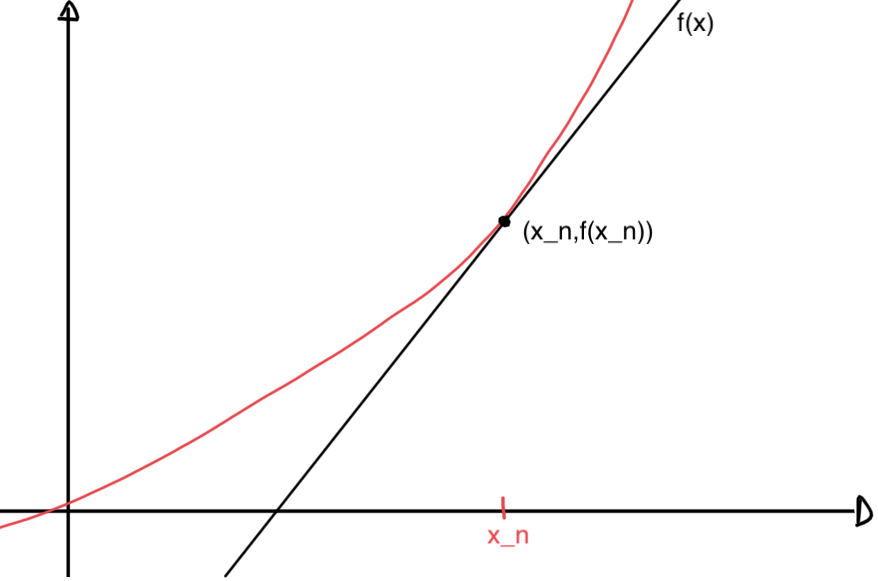
\includegraphics[width=0.5\textwidth]{immagini/approxNewtEs10.jpg}
	\caption{Approssimazione Esercizio 10.}\label{fig:approxNewtEs10}
\end{figure}

\noindent La retta tangente il grafico di $f(x)$ nel punto $(x_n, f(x_n))$ è $y-f(x_n)=f'(x_n)(x-x_n)$, essendo $f'(x_n)$ la derivata di $f(x).$ Ponendo $y=0$, è ricavata
\begin{equation*}
	x_{n+1}=x_n-\frac{f(x_n)}{f'(x_n)},\quad n=0,1,2,\hdots.
\end{equation*}

\noindent Dimostrare la convergenza quadratica ad una radice semplice di $ \overline{x}$ di $f(x)$ significa che $f'(x)\neq 0$, sotto ipotesi che $f\in C^{(2)}$ in un intorno di $\overline{x}$, per un opportuno intorno, per il Teorema della permanenza del segno, significa:
\begin{equation*}
	\begin{matrix}
		0&=&f(\overline{x})&=& f(x_n)+(\overline{x}-x_n)f'(x_n)+\frac{f''(\xi_n)}{2}(\overline{x}-x_n)^2&&\\
		&=&f'(x_n)\left(\boldsymbol{\frac{f(x_n)}{f'(x_n)}-x_n}+\overline{x}\right) + \frac{f''(\xi_n)}{2}(\overline{x}-x_n)^2&\overset{\footnotemark}{=}& f'(x_n)(x_{n+1}-\overline{x})+\frac{f''(\xi_n)}{2}(\overline{x}-x_n)^2\\
		&&&&\xi_n\in\underset{\footnotemark}{\uline{I(\overline{x}, x_n)}}
	\end{matrix}
\end{equation*}

\addtocounter{footnote}{-1}
\footnotetext{$\frac{f(x_n)}{f'(x_n)}-x_n$ è Newton al passo $n+1$, ovvero $x_{n+1}$.}

\stepcounter{footnote}
\footnotetext{Intervallo aperto nel quale gli estremi sono massimo e minimo. Se $x_n\rightarrow\overline{x}$ significa che anche $\xi_n\rightarrow\overline{x}$.}

\noindent Da questo segue che $f'(x_n)(\overline{x}-x_{n+1})=\frac{f''(\xi_n)}{2}(\overline{x}-x_n)^2.$ Ponendo $e_n=\overline{x}-x_n$ e dato che $f'(\overline{x})\neq 0$ è ottenuto ciò che segue: 
\begin{equation*}
	\frac{e_{n+1}}{e_n^2}=\frac{f''(\xi_n)}{2f'(x_n)}\longrightarrow\lim_{n\rightarrow\infty}\frac{|e_{n+1}|}{|e_n|^2}=\lim_{n\rightarrow\infty}\left|\frac{f''(\xi_n)}{2f'(x_n)}\right|=\left|\frac{f''(\overline{x})}{2f'(\overline{x})}\right|<\infty.
\end{equation*}

\paragraph{8.}\footnote{Slide 9 PDF 13.} Il numero di condizionamento di una radice è dato da $\boldsymbol{\frac{1}{|f'(\overline{x})|}}$, se $\overline{x}$ è la radice. In questo caso $f'(x)=3e^x+2\sin{(x)}\rightarrow f'(0)=3$. Pertanto, il numero di condizionamento della radice nulla di $f(x)$ vale $\boldsymbol{\frac{1}{3}}$

\paragraph{Osservazione sugli scritti:} Meglio scrivere ciò di cui siamo sicuri in termini di passaggi intermedi, altrimenti è meglio scrivere solo il risultato finale.

\paragraph{9.}\footnote{Slide 9 PDF 13.} La radice $\overline{x}$ di $f(x)=0$ ha molteplicità $m$ se:
$\begin{cases}
	f(\overline{x})=f'(\overline{x})=\hdots=f^{(\boldsymbol{m-1})}(\overline{x})=0,\\
	f^{(\boldsymbol m)}(\overline{x})\neq 0.
\end{cases}$

\noindent Se $\boldsymbol{m=1}$ la radice è \textbf{semplice}, se $\boldsymbol{m>1}$ la radice è \textbf{multipla}. La determinazione di una radice multipla è un problema malcondizionato, per il numero della radice, $\frac{1}{f'(\overline{x})}$, è infinito, essendo $f'(\overline{x})=0$. 

\noindent Data $f(x)=e^{x^2}-1\Rightarrow\boldsymbol{f(0)=0}$. Inoltre, $f'(x)=2xe^{x^2}\Rightarrow\boldsymbol{f'(0)=0}$ \footnote{Quindi, da qui, è possibile capire che la radice non è semplice.}. Ancora, $f''(x)=2e^{x^2}+4x^2e^{x^2}\Rightarrow\boldsymbol{f''(0)=2\neq 0}.$ Pertanto, la radice ha \textbf{molteplicità 2}.

\paragraph{10.} L'implementazione richiesta è nell'Algoritmo \ref{alg:polNewt}

\subsection{A.A. 2023/24}
\begin{enumerate}
	\item Approssimando $e=2.71828\hdots$ con $2.72$
	\begin{itemize}
		\item qual è l'errore assoluto commesso?
		\item qual è l'errore relativo?
	\end{itemize}
	\item Come si definisce la precisione di macchina di un'aritmetica finita? Qual è il suo significato?
	\item Dimostrare che, se $h\approx 0$, allora
	\begin{equation*}
		\frac{f(x+h)-f(x-h)}{2h}=f'(x)+o(h^2).
	\end{equation*}
	\item Cos'è il fenomeno della cancellazione numerica?
	\item Come si definisce l'ordine di convergenza di un metodo per la ricerca degli zeri di una funzione?
	\item Qual è il numero di massimo di iterazioni richiesto dal metodo di bisezione per determinare la radice di una funzione di cui sia noto l'intervallo di confidenza iniziale $[33,41]$, con accuratezza di $10^{-3}$?
	\item Derivare il metodo di Newton per la ricerca della radice di una funzione, e dimostrare che converge quadraticamente a radici semplici.
	\item Calcolare il numero di condizionamento della radice nulla di $f(x)=3\cos x-2-e^x$.
	\item Definire la molteplicità di una radice. Calcolare la molteplicità della radice nulla di
	\begin{equation*}
		f(x)=x\cos x - \sin x + \frac{x^3}{3}.
	\end{equation*}
	Perché il calcolo di una radice multipla è malcondizionato?
	\item Scrivere una function Matlab che implementi efficientemente il metodo	delle secanti.
\end{enumerate}

\hrule

\paragraph{1.}\footnote{Vedere Sezione \ref{sec:aritmetica_finita}.} L'errore assoluto è dato, se $x=e$ e $\tilde x=2.72$, da:
\begin{equation*}
	\Delta x=\tilde x - x = 2.72 - 2.71828\hdots \approx 2\cdot 10^{-3}.
\end{equation*}
Il corrispondente errore relativo è dato da:
\begin{equation*}
	\varepsilon_x = \frac{\Delta x}{x} = \frac{2 \cdot10^{-3}}{2.71828\hdots}\approx 7\cdot 10^{-4}.
\end{equation*}

\paragraph{2.} \footnote{Dal Teorema \ref{th:precisione_macchina_FL}.} Se si utilizza un'aritmetica finita in base $b$, con $m$ cifre per la mantissa, la corrispondente precisione di macchina è definita da:
\begin{equation*}
	u=
	\begin{cases}
		b^{1-m}, &\text{ in caso di troncamento},\\
		\frac{1}{2}b^{1-m}, &\text{ in caso di arrotondamento}.
	\end{cases}
\end{equation*}
Il suo significato è il seguente: dato $x\in\mathbb R$ e detto $fl(x)$ il corrispondente numero di macchina, se questo è normalizzato, allora la precisione macchina \gls{maggiora uniformemente} l'errore relativo di rappresentazione
\begin{equation*}
	\frac{|x-fl(x)|}{|x|}\leq u\quad (\text{se } x\neq 0).
\end{equation*}
$fl(x)$ è normalizzato se la prima cifra della mantissa è diversa da 0.

\paragraph{N.B.:} \textbf{È necessario conoscere la precisione macchina della singola e doppia precisione.}

\paragraph{3.}
\begin{itemize}
	\item $f(x+h)=f(x)+hf'(x)+\frac{h^2}{2}f''(x)+o(h^3)$,
	\item $f(x-h)=f(x)-hf'(x)+\frac{h^2}{2}f''(x)+o(h^3)$.
\end{itemize}
Sottraendo membro a membro, si ottiene:
\begin{equation*}
	f(x+h)-f(x-h)=2h\,f'(x)+o(h^3),
\end{equation*}
da cui, dividendo per $2h$, si ottiene
\begin{equation*}
	\frac{f(x+h)-f(x-h)}{2h}=f'(x)+o(h^2).
\end{equation*}

\paragraph{4.}\footnote{Vedere Sezione \ref{sssec:condizionamento_somma_algebrica}.} Questo fenomeno è la manifestazione del malcondizionamento della somma algebrica, in caso di addendi di segno discorde. Infatti, se $\tilde x_1 = x_1 (1+\varepsilon_1)$ e $\tilde x_2 = x_2 (1 + \varepsilon_2)$ sono gli addendi perturbati, allora $\tilde y = y (1 + \varepsilon_y)$ sarà il corrispondente risultato perturbato:
\begin{equation*}
	\begin{matrix}
		y &=& x_1 + x_2\\
		\tilde y &=& \tilde x_1 + \tilde x_2 &=& x_1(1+\varepsilon_1) + x_2 (1+\varepsilon_2) &=& \underbrace{x_1 + x_2}_{y} + x_1 \varepsilon_1 + x_2 \varepsilon_2.
	\end{matrix}
\end{equation*}
Da questo si ricava:
\begin{equation*}
	\boldsymbol{\varepsilon_y} = \frac{x_1\varepsilon_1+x_2\varepsilon_2}{x_1+x_2}= \boldsymbol{\frac{x_1\varepsilon_1+x_2\varepsilon_2}{y}},
\end{equation*}
da cui:
\begin{equation*}
	|\varepsilon_y|\leq \frac{|x_1|+|x_2|}{|x_1+x_2|} \cdot \max{\{|\varepsilon_1|,|\varepsilon_2|\}}.
\end{equation*}
Pertanto, il numero di condizionamento della somma algebrica è
\begin{equation*}
	\kappa=\frac{|x_1|+|x_2|}{|x_1+x_2|},
\end{equation*}
che non è limitato superiormente se $x_1$ e $x_2$ sono quasi opposti. In questo caso, il malcondizionamento del problema si manifesta, utilizzando un'aritmetica finita, nel fatto che, anche partendo da addendi con tutte le cifre significative corrette, si può ottenere un risultato con molte meno cifre significative corrette. (È possibile fare un esempio di malcondizionamento di una somma algebrica.)

\paragraph{5.}\footnote{Vedere Definizione \ref{def:ordine_convergenza_metodo_iterativo} Ordine di convergenza di un metodo iterativo.} Se consideriamo un metodo iterativo per determinare una conveniente approssimazione dello zero di una funzione, sia esso $x^*$, allora, dette $x_1, x_2,\hdots, x_n$ le apporssimazioni generate, il metodo avrà ordine di convergenza $p$ se, detto $e_n=x_n-x^*$ l'errore al passo $n$, si ha che  $p$ è il più alto valore per cui
\begin{equation*}
	\lim_{n\rightarrow\infty}\frac{|e_{n+1}|}{|e_n|^p}=c<+\infty.
\end{equation*}
$c$ si dice costante asintotica dell'errore.
\paragraph{N.B.:} È necessario conoscere l'ordine di convergenza dei metodi studiati.

\paragraph{6. }\footnote{Vedere Definizione \ref{def:itmax_metodo_bisezione}.} Ricordiamo che il metodo di bisezione approssima la soluzione col punto medio dell'intervallo di confidenza corrente. Pertanto, al passo $i$-esimo, l'errore sarà maggiorato da $2^{-i}$ per l'ampiezza dell'intervallo di confidenza iniziale. Nel nostro caso, $41-33=8=2^3$. Pertanto, richiedendo che
\begin{equation*}
	2^{-1}\cdot 2^3\leq 10^{-3}\approx 2^{-10},
\end{equation*}
si ottiene $2^{-i}\leq 2^{-13}$, ovvero $i=13$ passi.

\paragraph{7.}\footnote{Vedere Sezione \ref{ssec:metodo_newton} ed il Teorema \ref{th:metodo_newton_converge_quadraticamente}.} Il metodo di Newton si deriva ricercando, ad ogni iterazione, la radice dell'approssimazione lineare della funzione nel punto corrente. Se ci troviamo nel punto $x_1$, allora
\begin{equation*}
	f(x)\cong f(x_i)+(x-x_i)f'(x_i),
\end{equation*}
che è l'equazione della retta tangente al grafico di $f(x)$ in $(x_i, f(x_i))$.\\
Ricercando $x_{i+1}$ in modo tale che
\begin{equation*}
	f(x_i)+(x_{i+1}-x_i)f'(x_i)=0,
\end{equation*}
si ottiene:
\begin{equation*}
	x_{i+1}=x_i-\frac{f(x_i)}{f'(x_i)},\quad i=0,1,\hdots\, .
\end{equation*}
Per quanto riguarda la seconda parte, supponiamo $\boldsymbol{x_i\rightarrow\overline{x},\, i\rightarrow +\infty}$, radice semplice di $f(x)$. Pertanto, $\boldsymbol{f'(\overline{x})\neq 0}$. Si ottiene:
\begin{equation*}
	0=f(\overline{x})=f(x_i)+(\overline{x}-x_i)f'(x_i)+\frac{(\overline{x}-x_i)^2}{2}f''(\boldsymbol{\xi_i}),\quad \boldsymbol{\xi_i\in I(x_i,\overline{x})}.
\end{equation*}
Definendo $\boldsymbol{\overline{x}-x_i = e_i}$, l'errore al passo $i$, si ottiene, quindi:
\begin{equation*}
	\begin{matrix}
		0 &=& f(x_i)+(\overline{x}-x_i)f'(x_i)+\frac{(\overline{x}-x_i)^2}{2}f''(\xi_i) &=& \left[\overbrace{\frac{f(x_i)}{f'(x_i)}-x_i}^{-x_{i+i}} + \overline{x}\right]f'(x_i) + \frac{(\overline{x}-x_i)^2}{2} f''(\xi_i)\\
		&=& \underbrace{\left[\overline{x}-x_{i+1}\right]}_{e_{i+1}} f'(x_i) + \frac{(\overbrace{\overline{x}-x_i}^{e_i})^2}{2} f''(\xi_i) &=& e_{i+1} f'(x_i) + \frac{e_i^2}{2} f''(\xi_i).
	\end{matrix}
\end{equation*}
Pertanto,
\begin{equation*}
	\frac{|e_{i+1}|}{|e_i|^2}=\frac{1}{2}\frac{|f''(\xi_i)|}{|f'(\xi)|}\underset{i\rightarrow+\infty}{\longrightarrow}\frac{1}{2}\frac{|f''(\overline{x})|}{|f'(\overline{x})|},
\end{equation*}
che è finito, poiché $f'(\overline{x})\neq 0$. Pertanto, si ha convergenza quadratica.

\paragraph{Suggerimento:} Riguardare la derivazione del metodo di accelerazione di Aitken.

\paragraph{8.}\footnote{Vedere Definizione \ref{def:numero_condizionamento_radice} Numero di condizionamento di una radice.} Se $\overline{x}$ è la radice di $f(x)$, il suo numero di condizionamento è definito da
\begin{equation*}
	\kappa = \frac{1}{|f'(\overline{x})|}.
\end{equation*}
Nel nostro caso,
\begin{equation*}
	f'(x)=-3\sin x - e^x
\end{equation*}
e, quindi, $|f'(0)|=1$.\\
Il numero di condizionamento della radice nulla è $\kappa=1$.

\paragraph{9.}\footnote{Dalla Definizione \ref{def:radice_molteplicita_m} di radice di molteplicità $m$.} Diremo che $\overline{x}$ è radice di molteplicità $m$ di $f(x)$ se
\begin{equation*}
	f(\overline{x})=f'(\overline{x})=f''(\overline{x})=\hdots=f^{(m-1)}(\overline{x})=0,\, f^{(m)}(\overline{x})\neq 0.
\end{equation*}
La radice $\overline{x}$ si dice semplice se $m=1$, multipla se $m>1$.
\begin{equation*}
	\begin{matrix}
		m=0 & f(x) = x\cdot\cos x-\sin x + \frac{x^3}{3} & \rightarrow & f(0)=0 ;\\\\
		m=1 & f'(x) = \cancel{\cos x} - x \sin x - \cancel{\cos x} + x^2 & \rightarrow & f'(0)=0 ;\\\\
		m=2 & f''(x) = -\sin x - x\cos x + 2x & \rightarrow & f''(0)=0 ;\\\\
		m=3 & f'''(x) = -\cos x -\cos x + x\sin x  + 2 & \rightarrow & f'''(0)=0 ;\\\\
		m=4 & f^{(4)}(x) = 2\sin x + \sin x + x\cos x & \rightarrow & f^{(4)}(0)=0 ;\\\\
		m=5 & f^{(5)}(x) = 3\cos x + \cos x - x\sin x & \rightarrow & f^{(5)}(0)=4\neq 0 .
	\end{matrix}
\end{equation*}
Pertanto, la molteplicità della radice è $m=5$.\\
Il numero di condizionamento di $\overline{x}$, radice di $f$, è $\kappa = \frac{1}{|f'(\overline{x})|}$. Se la radice è multipla allora $f'(\overline{x})=0$ allora $\kappa=\infty$.

\paragraph{10.}\footnote{Vedere Sezione \ref{sssec:metodo_secanti}.} Il metodo delle secanti è un metodo a 2 passi definito dalla seguente iterazione:
\begin{equation*}
	\begin{matrix}
		x_{i+1} &=& x_i-\frac{f(x_i)}{\frac{f(x_i)-f(x_{i-1})}{x_i-x_{i-1}}} &=& x_i-(x_i-x_{i-1})\cdot\frac{f(x_i)}{f(x_i)-f(x_{i-1})}&=&\\\\
		&=& x_i-\frac{f(x_i)(x_i-x_{i-1})}{f(x_i)-f(x_{i-1})} &=& \frac{x_{i-1}f(x_i)-x_i f(x_{i-1})}{f(x_i)-f(x_{i-1})},\quad i=1,2,\hdots.
	\end{matrix}
\end{equation*}

Per l'implementazione vedere l'Algoritmo \ref{alg:metodo_secanti}.